% !TeX spellcheck = cs_CZ
\begin{example}\label{TEO:ex_InvOpamp01}
  Uvažujme invertující zesilovač s ideální operačním zesilovačem typu VFA s naznačenými uzly 
  tak, jak je na obr. \ref{TEO:fig_MMUN_inv_opamp}. Napište rovnice MMUN.
  
   {\centering
    \captionsetup{type=figure}
    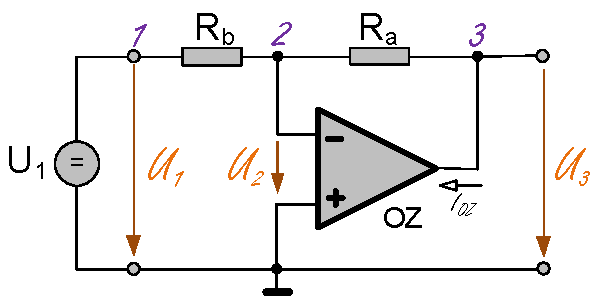
\includegraphics[width=0.7\linewidth]{MMUN_inv_OPAMP.pdf}
    \captionof{figure}{Invertující zesilovač}
    \label{TEO:fig_MMUN_inv_opamp}
    \par}
  
  Rovnice MMUN budou v maticovém zápisu vypadat takto:

    % using \usepackage{array} and command \newcolumntype{C}[1]{>{\centering}m{#1}}!
   {\centering
    \begin{tabular}{|C{0.6cm}|C{1.2cm}|C{0.6cm}|C{0.45cm}|C{0.45cm}|C{.3cm}|c|C{.33cm}|c|}
        \multicolumn{1}{c}{$U_1$}    & \multicolumn{1}{c}{$U_2$}    & \multicolumn{1}{c}{$U_3$}  & 
        \multicolumn{1}{c}{$I_1$}    & \multicolumn{1}{c}{$I_{OZ}$} & \multicolumn{1}{c}{ }      &  
        \multicolumn{1}{c}{x}        & \multicolumn{1}{c}{ }        & \multicolumn{1}{c}{b}       \\
      \cline{1-5}\cline{7-7} \cline{9-9}
      $G_b$  & $-G_b$    &  & -1  &  & \multirow{5}{*}{$\ast$} & $U_1$ & \multirow{5}{*}{=}     & \\
      \cline{1-5} \cline{7-7} \cline{9-9}
      $-G_b$ & $G_a+G_b$ & $-G_a$ &  &   & & $U_2$      &      &                                  \\
      \cline{1-5} \cline{7-7} \cline{9-9}
             & $-G_a$    & $G_a$  &  & 1 & & $U_3$      &      &                                  \\
      \cline{1-5} \cline{7-7} \cline{9-9}
         1   &           &        &  &   & & $I_1$      &      &    $U_{IN}$                      \\
      \cline{1-5} \cline{7-7} \cline{9-9}
             &     1     &        &  &   & & $I_{OZ}$   &      &                                  \\
      \cline{1-5} \cline{7-7} \cline{9-9}
    \end{tabular}
    \par}
  \vspace{1em}
  Předposlední rovnice říká, že uzlové napětí $U_1$ je rovno napětí signálového zdroje $U_{IN}$. 
  Jednička v posledním řádku reprezentuje jednoduchou rovnici $U_2 = 0$. Ačkoliv je obvod poměrně 
  jednoduchý, je pro ruční řešení neefektivní, neboť jsme získali soustavu o 5 rovnic a 5 neznámých.
\end{example}